\section{Introduction}
\label{sec:intro}
Building sector accounts for 30\% of the total energy consumption and 26\% of the energy-related CO2 emissions \cite{IEA2023}, therefore seeking energy efficiency measures for buildings is a key aspect in the energy transition (\cite{EEb2020}). Optimal operation of buildings through advanced control strategies has appeared to reduce both the energy consumption and CO2 emissions of buildings \cite{Stoffel2023}. Among the various advanced building control techniques that can be found in the literature, Model Predictive Control (MPC) is the most widely used one since it can achieve energy savings while improving the thermal comfort making use of a mathematical model of the buildings to predict its performance considering the weather and occupancy forecast and calculating the optimal actuation \cite{Taheri2022}. Many examples of MPC applied to pilot buildings can be found in the literature, which have demonstrated energy savings from 15\% to 50\% \cite{Drgona2020}, but its implementation in real life is still in a very early stage. Most of the authors that have performed extensive reviews on MPC works that can be found in the recent years’ literature \cite{Yao2021}, \cite{Ahmad2021} \cite{Taheri2022} agree that the modeling approach for the MPC is one of the key decisions. In this regard, there are three possible approaches: $white-box$, $black-box$ and $grey-box$ modeling \cite{Kim2022}. White-box approach models the building dynamics and controlled units using physical equations. It typically produces accurate and detailed models, but at the expense of a high computational cost that may be prohibitive for the implementation \cite{Yu2022}.On the contrary, the black-box model relies exclusively on models that are driven by data, neglecting physical equations \cite{Hauge2022}.  While this approach is computationally efficient, it might be lacking for explanatory power. Finally, grey-box modeling appears as an in-between solution, which combines physical equations with parameters to be calibrated with real data \cite{Kumar2023}. This approach is the most widely used approach in MPC \cite{Serale2018}. Furthermore, alternative approaches, including MPC hierarchisation \cite{Raghuraman2020}, have been examined as potential reductions in computational cost, alongside the modelling approach. This enables the problem to be decomposed into distinct subsystems; however, it was determined in \cite{Camponogara2021} that a control system that takes into account the entire plant is still required to optimize performance.

Another challenging aspects of MPC is the inherent uncertainty of the problem due to the unknown time-variant physical characteristics of the building \cite{Maasoumy2014}; the uncertain occupancy, which generate internal heat gains that affect the climate demand \cite{}; and the uncertainty in the weather predictions used by the MPC \cite{Oldewurtel2012}. In this regard, Moving Horizon Estimator (MHE) is an estimation technique that has proven to  improve state estimates for optimization and control \cite{Hedengren2017}. This technique has been applied in \cite{Simmons2019} to re-calibrate the building model parameters based on the latest measurements and calculate the unknown variables. This approach for the MPC implementation was also tested in \cite{Gates2021} for a whole building management, in \cite{Kim2018} for a commercial building. In \cite{Zabala2023} an MPC integrating the MHE was compared to a fixed-parameter MPC, and the MPC integrating the MHE improved the targets.

Other alternatives to MPC were studied, mainly reinforcement learning (RL). Reinforcement Learning is a black box method that learns the control strategy automatically from experience in a real or simulated environment \cite{Belyadi2021}. It doesn’t require expert intervention, however it also does not allow it when expert intervention is desirable. Some studies of RL applied to buildings can be found in the literature, but the number is very limited compared to the MPC studies. Some remarkable examples are \cite{Arroyo2022} which compares the performance of RL and MPC, but the results reached with the MPC are more promising; and \cite{Stoffel2023} in which a quantitative and qualitative comparison is performed including aspects as adaptability or interpretability. 

Automatic program synthesis is an approach that has been studied since the dawn of computer science \cite{Balzer1985}, but has recently seen many breakthroughs due to the advent of Large Language Models. It combines the explainability and expert knowledge injection advantages of MPC with the data-driven nature of reinforcement learning: a neural network generates a piece of human-readable and editable code that controls an agent and updates the code as the agent gets positive or negative feedback on its performance. Methods that can generate problem-solving programs without human intervention are new and their applications to real-world problems remains largely unexplored, with a possible exception of spreadsheet autocompletion where systems like FlashFill \cite{Gulwani2011} are already built into consumer products.

One of the main challenges when addressing the performance of this type of advanced control strategies is performing a fair comparison among them. Most of the research studies found in the literature demonstrate the improved operation of the building with the optimized technique individually, against a certain baseline scenario. But comparison among different advanced control techniques and developed case studies is lacking. In this regard, the Building Optimization Testing Framework (BOPTEST) \cite{Blum2021} was developed to address this challenge and provide a simulation-based benchmarking platform to compare the control algorithms on some common emulators.

\subsection{Contributions of the chapter}
\label{sec:contribution}
The contributions of this chapter, with respect to the literature and previous studies, are:
\begin{itemize}
  \item Implementation of an Model Predictive Control with the Moving Horizon Estimator technique for online recalibration of the model and internal heat gains estimation.
  \item Application of program synthesis with large language models to the control of a building.
  \item Addressing and comparing the performance of two advanced control strategies using a benchmarking framework, having a preliminary assessment/comparison between the most predominant advanced control technique (MPC) and a promising one (Program synthesis) considering results on other fields.
\end{itemize}

\subsection{Organization of the chapter}
Section \label{sec:organization}
The chapter is organized as follows. Section \ref{sec:method}  describes the emulator from BOPTEST that is chosen for the comparison, the implementation of the MPC problem for the building and the application of program synthesis with large language models. Section \ref{sec:results} shows the results of the comparison of the MPC and the program synthesis with emulator of the BOPTEST. Section \ref{sec:discussion} analyses the simulation results and KPI comparison, and presents the advantages and limitations of each approach. Finally, section \ref{sec:conclusion} reports on the conclusions and future research.

\section{Method}
\label{sec:method}
This section first describes the test case from the BOPTEST framework selected to perform a comparison and assessment of both advanced control strategies. Then, the implementation of the Model Predictive Control is described, including the embedded reduced order model of the building and the heat pump, and the Moving Horizon Estimation technique description, which is used for the real-time calibration of the model. Finally, the Program Synthesis implementation through large language models is presented.


\subsection{BOPTEST framework for benchmarking}
\label{sec:BOPTEST}
The Building Optimization Testing (BOPTEST) framework \cite{Blum2021} is used for a fair evaluation and benchmarking of both control solutions. The framework provides a simulation environment with different emulator buildings with boundary conditions (weather and electricity pricing) and baseline controllers. The simulation framework provides a series of Key Performance Indicators (KPI) that can be used to address the performance.

In this study, the BESTEST Hydronic Heat Pump emulator is selected. This emulator represents a residential dwelling of 192 m2 for a family of 5 members located in Brussels (Belgium).  The heating system, depicted in \ref{fig:1}, is composed of a 15 kW air-to-water modulating heat pump to absorb energy from the surrounding air in order to heat the floor heating system. During the operation of a heat pump, the evaporator fan facilitates the circulation of ambient air through the heat pump evaporator. The floor heating system uses water as the working fluid to transfer heat into the floor. The building envelope model is implemented using the IDEAS library \cite{Jorissen2018}. The rectangular floor plan is 12 m by 16 m. Internal walls are configured such that there are around 12 rooms in the building. The building further contains 24 m2 of windows on the south facade.

% For one-column wide figures use
\begin{figure}
% Use the relevant command to insert your figure file.
% For example, with the graphicx package use
  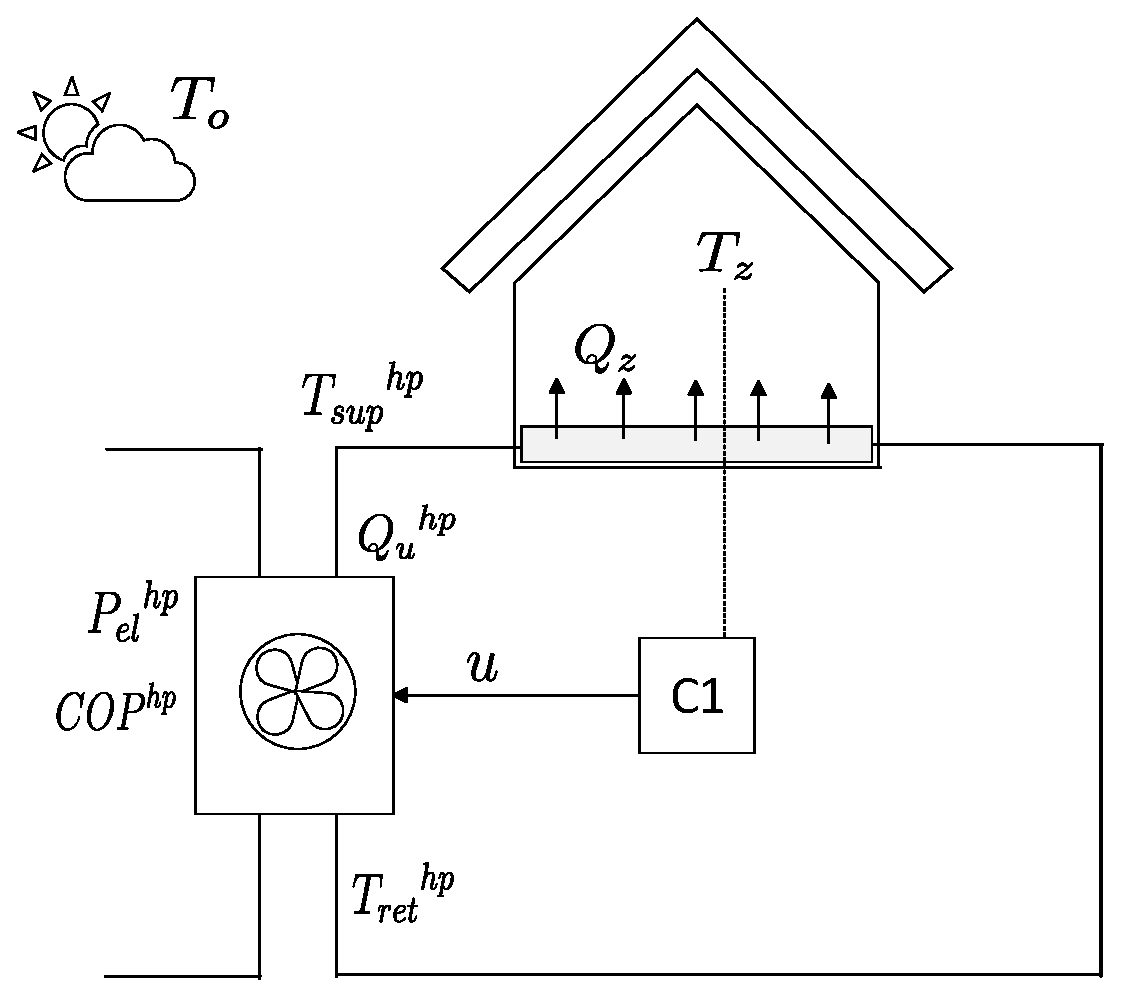
\includegraphics[scale=.4]{boptest/Fig1.eps}
 % figure caption is below the figure
\caption{Bestest hydronic heat pump test case system schematic.}
\label{fig:1}       % Give a unique label
\end{figure}
%

Figure \ref{fig:1} shows an schematic of the bestest hydronic heat pump emulator, reflecting the variables that are considered for this study. Regarding the variables from the indoor thermal zone, $T_{z}$ is the indoor temperature of the thermal zone and $Q_{z}$ is the input heat from the radiant floor to the house. The heat pump modulation signal for compressor frequency can be manipulated and is represented by $u$. The heat pump variables considered in the study are the supply heat pump temperature ${T_{sup}}^{hp}$, the return heat pump temperature ${T_{ret}}^{hp}$, the heat supplied by the heat pump ${Q_{u}}^{hp}$, the heat pump electric consumption ${P_{el}}^{hp}$, and the heat pump coefficient of performance $COP^{hp}$. A baseline controller consisting of a PI with the indoor temperature as the controlled variable and the heat pump modulation signal for compressor frequency as the control variable is also available to be used as baseline. This baseline controller is reprented by C1 in Figure \ref{fig:1}, and is the controller that is replaced by the MPC or the program generated by program synthesis. All other equipment (fan for the heat pump evaporator circuit and floor heating emission system pump) are switched on when the heat pump is working (modulating signal higher than 0) and switched off otherwise, with an additional controller. Finally, $T_o$ is the outdoor dry bulb temperature for the location.

Two different testing periods are available for this emulator:
\begin{itemize}
    \item $The peak heat day period$. A two-week testing period preceded by a one.week warmup period during which the baseline control is utilized. The two weeks for testing are centered arounf the day of the year that experiences the highest 15-minute system heating demand. This period runs from day 16 to day 30 of the year.
    \item $The typical heat day period$. This testing period also spans two weeks and includes a one-week warmup phase of one additional week. The two testing weeks, running from day 108 to day 122 of the year, is centered on the day with the highest 15-minute system heating load that is nearest, but not exceeding, the median of all 15-minute maximum heating loads throughout the year.
\end{itemize}
Regarding the energy pricing, there are three pricing scenarios: 
\begin{itemize}
    \item $Constant electricity price$. The constant electricity pricing scenario employs a fixed rate of 0.0535 EUR/kWh, sourced from the "Easy Indexed" electricity deal (standard rate) available at https://www.energyprice.be/products-list/Engie \cite{Engie}.  The total electricity price, including transmission fees and taxes, is 0.2535 EUR/kWh.
    \item $Dynamic electricity price$. The dynamic electricity pricing model employs a dual rate structure, with a rate of 0.0666 EUR/kWh during the day and 0.0383 EUR/kWh during the night. This information was acquired from the "Easy Indexed" electricity deal (dual rate) available at \cite{Engie}.   The on-peak daily time occurs from 7:00 a.m. to 10:00 p.m.   The off-peak daily time occurs from 10:00 p.m. to 7:00 a.m.  The total power prices, including transmission fees and taxes, amount to 0.2666 EUR/kWh during on-peak periods and 0.2383 EUR/kWh during off-peak periods.
    \item $Highly dynamic electricity price$. The power price scenario is determined by the day-ahead energy prices in the BELPEX wholesale electricity market in Belgium during the year 2019 \cite{Elexys}.  It should be noted that the prices mentioned above are subject to additional charges in the form of constant gearbox fees and taxes, which amount to 0.20 EUR per kilowatt-hour.
\end{itemize} 
The profile of the Electricity Emissions Factor considered in this test case is a constant emission factor of 0.167 kgCO2/kWh, which corresponds to the grid power emission factor provided by the Association of Issuing Bodies (AIB) for the year 2018. 

\subsection{Model Predictive Control}
\label{sec:MPC}
The MPC is implemented together with the MHE technique, and its calculated outputs are simulated in BOPTEST emulator following the configuration shown in Figure \ref{fig:2}.

% For one-column wide figures use
\begin{figure}
% Use the relevant command to insert your figure file.
% For example, with the graphicx package use
  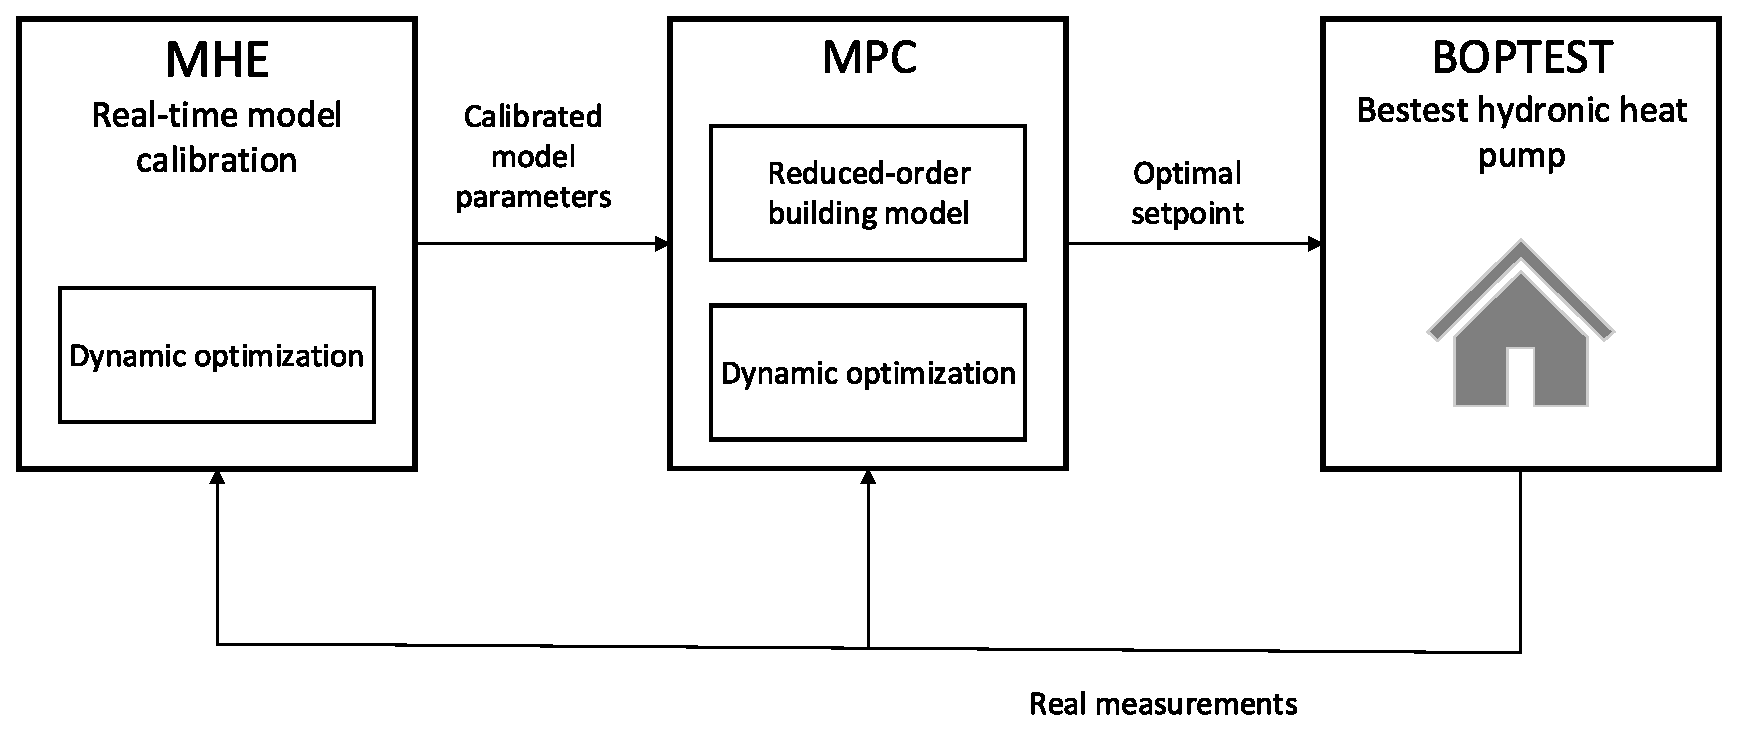
\includegraphics[scale=.4]{boptest/Fig2.eps}
 % figure caption is below the figure
\caption{Model Predictive Control implementation scheme with BOPTEST.}
\label{fig:2}       % Give a unique label
\end{figure}
%

As stated in Section \ref{sec:intro}, the model embeded in the MPC is a key aspect. So first, the reduced order model of the building and the heat pump are described. Then, the MPC problem is defined, and finally the implementation of the MHE is exposed.

\paragraph{Reduced order building model integrated in the MPC} 

The system model incorporated in an MPC plays a crucial role in its development, since the accuracy of the model directly affects the reliability of system predictions and the achievement of control and optimization objectives. One of the main challenges lies in achieving a balance between the precision of the model, which accurately and comprehensively represents the intricacies and dynamics of the system, and the computational load. This is important as the optimization problem needs to be solved within a timeframe that enables real-time implementation, as is the case for the application discussed in this chapter, where updates are required every 15 minutes.
The model embedded in the MPC considers two main components. First, a model of the thermal zone that represents the indoor of the house, and secondly the heat pumps model.
Regarding the indoor house model, it considers many factors including the thermal building envelope, internal heat gains, and heat losses resulting from heat conduction, convection, and ventilation. Modelling is supported by the utilization of calibrated reduced-order data-driven grey box models. The employed grey-box model is derived from a Resistance-Capacitance (RC) network, as described in \cite{Kim2018_2}, to represent a thermal zone. This model takes into account the relevant physical properties and disturbances associated with unmeasured inputs. Nevertheless, it can be calibrated using other measured variables. The experimental demonstration of the model's performance has been presented in the referenced literature \cite{Kim2016}.

The topology of a single thermal zone is depicted in Figure \ref{fig:3}, showing the embedded RC network model structure. The thermal zone refers to a designated space that is regulated by a thermostat and served by a heating source. The variable $T\textsubscript{z}$ denotes the temperature of the indoor zone, whereas $T\textsubscript{w}$ represents the temperature of the walls, roof, and floor, collectively characterizing the thermal behavior of the enclosures. The variable $T\textsubscript{o}$ represents the outdoor ambient temperature of the surrounding external environment. The thermal capacitances of the zone and wall are denoted as $C\textsubscript{z}$ and $C\textsubscript{w}$, whereas the thermal resistances between the zone air and wall, and between the zone air and external air, are represented by $R\textsubscript{zw}$ and $R\textsubscript{zo}$, respectively. The variable $Q\textsubscript{g}$ denotes internal heat gains that have not been quantified. $Q\textsubscript{z}$ refers to the input heat by the radiant floor heating system.

% For one-column wide figures use
\begin{figure}
% Use the relevant command to insert your figure file.
% For example, with the graphicx package use
  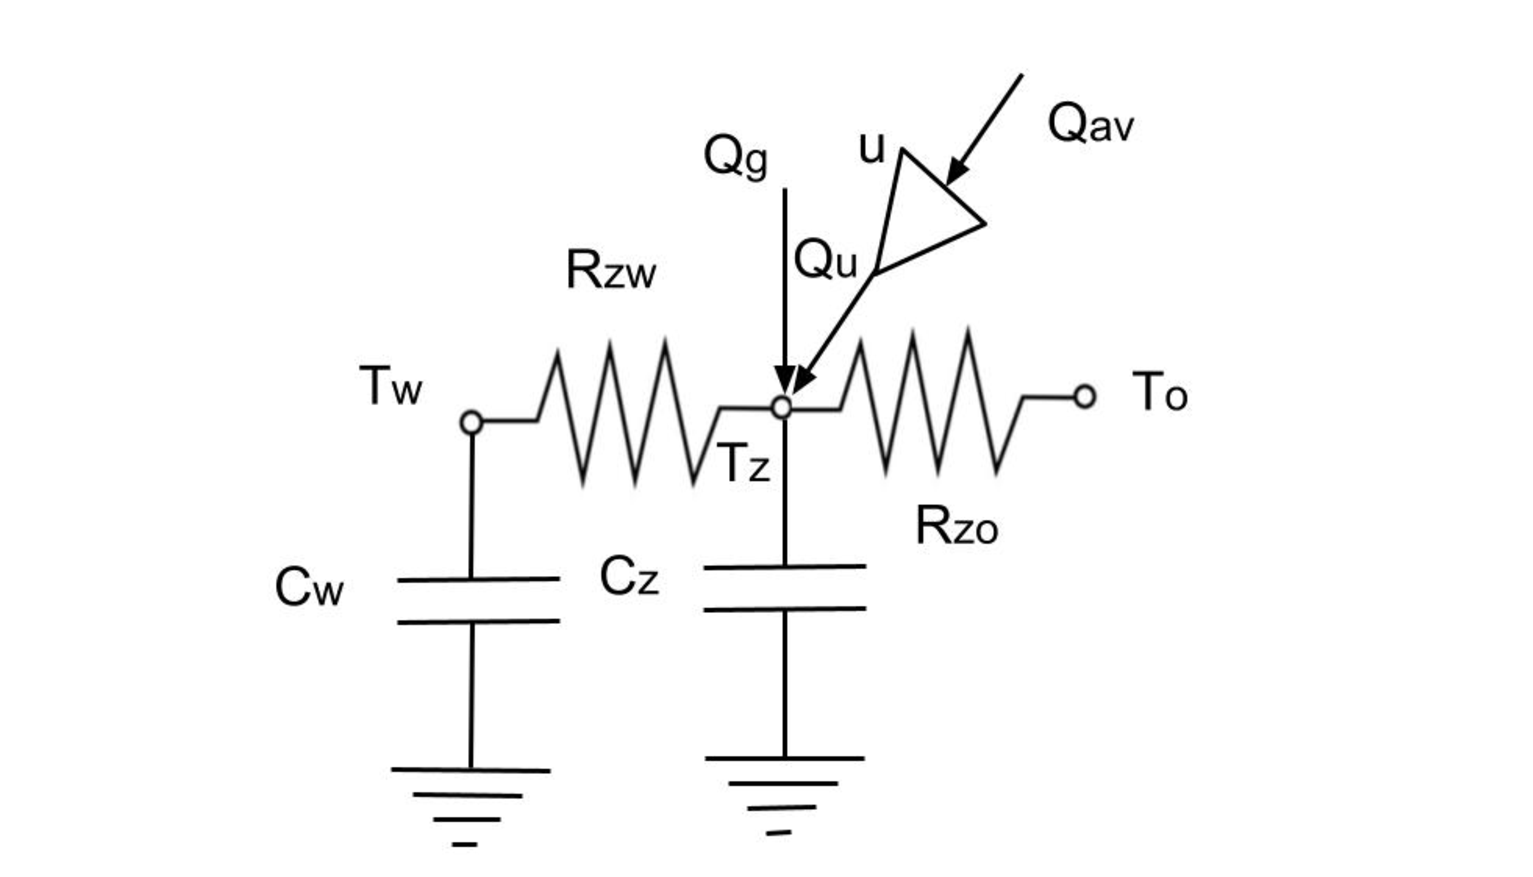
\includegraphics[scale=.4]{boptest/Fig3.eps}
% figure caption is below the figure
\caption{Reduced order Resistance-Capacitance model for building}
\label{fig:3}       % Give a unique label
\end{figure}
%

Equations \ref{eq:1} and \ref{eq:2} are the differential equations for the thermal balance in the zone.
\begin{equation}
C_z \cdot \frac{dT_z}{dt} = \frac{T_w-T_z}{R_{zw}} + \frac{T_o-T_z}{R_{zo}} + Q_g + u \cdot Q_{av}
\label{eq:1}
\end{equation}

\begin{equation}
C_w \cdot \frac{dT_w}{dt}=\frac{T_z-T_w}{R_{zw}}
\label{eq:2}
\end{equation}

In the case of the air-to-water electric heat pump, the corresponding EnergyPlus model is used (\cite{EnergyPlus}). The electric consumption of the heat pump ($P\textsubscript{el}\textsuperscript{hp}$) depends on the supply temperature of the water leaving the heat pump ($T\textsubscript{sup}\textsuperscript{hp}$), the outdoor temperature ($T\textsubscript{o}$) that enters the heat pump and the part-load ratio ($PLR$) at which the heat pump is working. The electric consumption is calculated using Eq. \ref{eq:3}:

\begin{equation}
P_{el}^{hp} = (Q_{av} \cdot EIRFT \cdot EIRFPLR)/COP_{ref}
\label{eq:3}
\end{equation}

$Q_{av}$ is the available load side capacity, EIRFT is the energy input ratio (EIR) modifier curve at full load, EIRFPLR is the EIR modifier curve at part load and $COP_{ref}$ is the reference COP at maximum load. 

The available load capacity is computed by Eq. \ref{eq:4}:
\begin{equation}
P_{el}^{hp} = (Q_{av} \cdot EIRFT \cdot EIRFPLR)/COP_{ref}
\label{eq:4}
\end{equation}

CAPFT is the capacity modifier function and is computed by Eq. \ref{eq:5}, which accoridng to DOE2 is a polynomic curve:

\begin{equation}
CAPFT = f(T_{sup}^{hp},T_{o}) = a_0 + a_1 \cdot {T_{sup}}^{hp} + a_2 \cdot {{T_{sup}}^{hp}}^2 + a_3 \cdot T_{o} + a_4 \cdot T_{o}^2 + a_5 \cdot {T_{sup}}^{hp} \cdot T_o
\label{eq:5}
\end{equation}

EIRFT is based on both temperatures and is computed by Eq. \ref{eq:6}, having a polynomic shape:

\begin{equation}
EIRFT = f(T_{sup}^{hp},T_{o}) = b_0 + b_1 \cdot {T_{sup}}^{hp} + b_2 \cdot {{T_{sup}}^{hp}}^2 + b_3 \cdot T_{o} + b_4 \cdot T_{o}^2 + b_5 \cdot {T_{sup}}^{hp} \cdot T_o
\label{eq:6}
\end{equation}

EIRFPLR depends on the PLR and is calculated by Eq. \ref{eq:7}:

\begin{equation}
EIRFPLR = f(PLR) = c_0 + c_1 \cdot PLR + c_2 \cdot PLR^2
\label{eq:7}
\end{equation}

PLR is calculated by Eq. \ref{eq:8}:

\begin{equation}
PLR = \frac{{Q_{u}}^{hp}}{Q_{av}}
\label{eq:8}
\end{equation}

${Q_{u}}^{hp}$ is the thermal load supplied by the heat pump. It is assumed that the PLR is directly proportional to the modulation signal $u$ that controls the compressor frequency.  

The model of the entire system is based on the assumption that the heat supplied by the heat pump ${Q_{sup}}^{hp}$ is equal to the input heat to the indoor thermal zone by the radiant floor $Q_z$, that is, the distribution circuit and the heat transfer at the radiant floor are assumed to be ideal with no heat losses.

\paragraph{Model Predictive Control problem definition} The MPC is implemented through the following dynamic optimization problem:

\begin{equation}
min w_{T_z}^T \cdot e_{T_z} + w_{cost}^T \cdot cost
\label{eq:9.a}
\end{equation}

subject to:
\begin{equation}
0=f(\frac{dx}{dt},x,y,u)
\label{eq:9.b}
\end{equation}
\begin{equation}
0\leq g(\frac{dx}{dt},x,y,u)
\label{eq:9.c}
\end{equation}

The cost function of the MPC dynamic optimization problem is presented in Eq. \ref{eq:9.a}, which is the sum of the error in the indoor temperature $T\textsubscript{z}$ compared to the upper and lower thermal comfort limits, defined in the BOPTEST emulator, and the total energy cost. The error in the temperature is computed using the I1-norm, that is, the absolute difference between the current measured value and the desired target value. Even if this operator does not have a continuous first and second derivative at $x=0$, the GEKKO software used for the problem definition handles the problem in a way that this discontinuity is avoided, as explained in \cite{Hedengren2017}. The energy cost is computed considering the electric power consumption of the heat pump and the dynamic electricity price. Both objectives prioritization is controlled by tunning the weighting factors $w\textsubscript{T\textsubscript{z}}$ and $w\textsubscript{Cost}$.

Equation \ref{eq:9.b} represents the equality constrains of the problem, derived from the building model, and Equation \ref{eq:9.c} represents the inequality constrains, used to impose physical limits to the variables.

The variable $x$ denotes the state variables, that is, both the indoor and wall temperatures, so $x=[T\textsubscript{z},T\textsubscript{w}]$. The manipulated variable is the heat pump compressor speed u, and y represents the power consumption of the heat pump. 

The real measurements used by the MPC are the indoor temperature $T_z$, and the supply and return temperatures of the heat pump, that is used to calculate the available heat for the room. The predictions used by the MPC are the outdoor dry bulb temperature forecast, and the internal heat gains estimated by the MHE.

The MPC is built to work with a prediction horizon of 12 hours and an actuation time of 15 minutes.

\paragraph{Model calibration approach}
The BOPTEST allocates an additional week for each scenario, preceding the two weeks designated for testing, which may be utilized for warm-up purposes. With regard to the MPC, two duties are completed this week:
\begin{itemize}
  \item $Model calibration for the heat exchanger$. The model parameters for the heat pump exhibit less time variation compared to those for the thermal zone; therefore, it is possible to train and maintain these parameters constant for the MPC application. Thus, the heat pump model is calibrated during the warm-up period. Utilising the methodology described in \cite{Monfet2013}, the parameters of the equations \ref{eq:5}, \ref{eq:6}, and \ref{eq:7} are computed. 
  \item $Pre-calibration of the RC models for the thermal zone$. The parameters of the RC thermal zone model are updated using the MHE; however, this model requires an initial value to start with at the first instants. These values serve as the model's initial values, and parameter updates are performed in accordance with them; therefore, it is crucial to have an accurate initial value. During the warm-up phase, initial values for the RC parameters that are practical and appropriate for the case under investigation are determined.
\end{itemize}

The calibration of the RC model parameters is then enhanced by means of an online re-calibration facilitated by the MHE.
The refence value used by the MHE as input to calibrate the model is the indoor zone temperature. Other variables that are assumed to be measured are the supply and return temperature of the heat pump, the modulation signal of the heat pump and the outdoor temperature.

\paragraph{Moving Horizon Estimator for model recalibration} Moving Horizon Estimator (MHE) is an estimation technique implemented through a dynamic optimization problem that seeks to minimize the difference between the real measurements of a system and the values derives with the prediction model. Moreover, a set of constraints can be added. The problem can be formulated through a dynamic optimization as follows:

\begin{equation}
min w_{T_z}^T \cdot e_{T_z} + w_{P}^T \cdot P
\label{eq:10.a}
\end{equation}

subject to:
\begin{equation}
0=f(\frac{dx}{dt},x,y,u)
\label{eq:10.b}
\end{equation}
\begin{equation}
0\leq g(\frac{dx}{dt},x,y,u)
\label{eq:10.c}
\end{equation}

The objective function is represented in Eq. \ref{eq:10.a} and aims to minimize the difference between the real indoor temperature and heat pump power consumption values compared to the reduced order model that wants to be calibrated. Equations \ref{eq:10.b} and \ref{eq:10.c} denote the equality and inequality constrains respectively, which are used to integrate the model of the thermal zone described in \ref{sec:MPC} and stablishes physical variables. The outputs of the MHE are the model parameters, $R\textsubscript{zo}$, $R\textsubscript{zw}$, $C\textsubscript{z}$, $C\textsubscript{w}$. 
The MHE is also used to estimate the internal heat gains in the thermal zone, denoted as $Q_g$. This estimation is used by the MPC as a prediction of the internal heat gains for the next hours. 

\paragraph{Software for MPC implementation} Python 3.11 is employed to address this particular development. The implementation of the MHE and MPC algorithms has been carried out using the GEKKO library \cite{Beal2018} in the Python programming language. This library is built upon the APMonitor framework \cite{Hedengren2014}. The solver employed in this study is IPOPT.

\subsection{Program synthesis with large language models}
\label{sec:ProgramSynthesis}
The program synthesis approach is implemented with a Synthesize Execute Instruct Debug loop over GPT-4 \cite{GPT2023} language model. This approach has demonstrated its ability to tackle programming challenges in \cite{Reflexion2023,teaching2023,Fully2023}, however two modifications are applied to adapt it to the building optimization domain:

\begin{enumerate}
  \item A chat language model is used as opposed to an instruction-driven language model. Unlike the instruction-driven approach, the chat-driven approach includes previous candidate solutions into the language model’s context window as additional information to guide generation and, in particular, avoid repeating mistakes. This advantage has prompted the developers of newer code generation models, such as GPT-4 and CodeLLAMA \cite{Code2023}, to operate in the chat paradigm.
  \item BOPTEST is an interactive environment with several continuous KPIs, namely, thermal discomfort and energy cost, while \cite{Reflexion2023,teaching2023,Fully2023} only experiment with pass/fail test cases.
\end{enumerate}
The SEID loop for BOPTEST case is as follows:
\begin{enumerate}
  \item A text description of the problem is provided. A verbatim copy of the reference document for the BESTEST Hydronic Heat Pump emulator is used, followed by a line of text explaining in which format the program can communicate with the environment (via standard input and output streams). This description is inserted into the first message of a simulated chat with a programming assistant.
  \item A continuation of the chat is sampled from the large language model.
  \item A candidate solution is extracted from the first code block in the assistant’s response.
  \item The candidate gets to control the thermostat in BOPTEST environment for a full episode (see below). The program receives current indoor temperature, $T_z$, and 12 hour forecasts for outside temperature, $T_o$, and electricity cost as input and is expected to output the heat pump modulating signal $u$.
  \item A report of the control episode is saved, including the KPIs (thermal discomfort, energy use, energy cost, CO2 emissions) and a timeline of:
  \begin{enumerate}
      \item The indoor temperature, $T_z$, in Kelvin.
      \item Heat pump modulating signal $u$ (0-1).
      \item Heat pump electrical power ${P_{el}^{hp}}$.
      \item Supply water temperature to radiant floor ${T_{sup}^{hp}}$.
      \item Return water temperature from radiant floor ${T_{ret}^{hp}}$.
  \end{enumerate}
  \item If the timeline is too long to fit into the context window of a language model, the timeline is resampled with average pooling, i.e. an N is selected and every N subsequent observations are replaced with their mean values.
  \item Another language model is used to summarize the report and generate a text report of the control episode. The values of all KPIs are appended to the text report.
  \item The report is appended to the chat along with a request to assistant "\textit{Can you rewrite the program to lower the costs and/or discomfort?}".
  \item Go to step 2.
\end{enumerate}

In this chapter’s experiments both the coding assistant language model and the report summarization language model are GPT-4.

The same testing scenario is used as in the MPC case, however, preliminary experiments have shown that running the full 7 day experiment at each iteration of the feedback loop is not necessary to achieve convergence. Instead, the control episodes are truncated to a shorter time period according to the following truncation schedule shown in Table \ref{tab:1}.

% For tables use
\begin{table}
% table caption is above the table
\caption{Truncation Schedule}
\label{tab:1}       % Give a unique label
% For LaTeX tables use
\begin{tabular}{lllllllllll}
\hline\noalign{\smallskip}
itearation & 1 & 2 & 3 & 4 & 5 & 6 & 7 & 8 & 9 & 10 \\
\noalign{\smallskip}\hline\noalign{\smallskip}
len, hours & 0.5 & 1 & 2 & 4 & 8 & 16 & 32 & 64 & 128 & 169 \\
\noalign{\smallskip}\hline
\end{tabular}
\end{table}

This way, as candidate solutions get more mature and sophisticated, they are tested more thoroughly and minor imperfections can be detected.

\section{Results}
\label{sec:results}
The MPC and the program generated by program synthesis with large language models are simulated using the BOPTEST testbed hydronic heat pump emulator for all the available scenarios, combining the both demand periods (peak heat day period and typical heat day period) with the three energy pricing scenarios (constant, dynamic and highly dynamic). For each scenario, the second week is chosen for testing, that is, from day 23 to 30 in the peak heat period, and between days 115 and 122 for typical heat day period.
For each scenario, the KPIs provided by the BOPTEST framework are evaluated.
 \begin{enumerate}
     \item $Thermal discomfort$: describes the cumulative deviation of indoor zone temperature from upper and lower thermal comfort limits. These comfort limits are defined for the selected emulator.
     \item $Energy use$: corresponds the heat pump energy use.
     \item $Cost$: reports the operational cost associated with the heat pump energy usage considering the pricing.
     \item $Emissions$: defined the CO2 emissions from the heat pump energy use.
 \end{enumerate}
 
The KPIs on which the results analysis will focus are the thermal discomfort and energy cost, as they assess the performance of the controllers for the two defined objectives: guarantee thermal comfort and minimize the energy cost.

The results will be divided by the two analyzed periods: typical heat day period and peak heat day period.

In the case of program synthesis, the program is generated using the most demanding conditions, that is, the peak heat day period with highly dynamic price scenario. The winning program generated for this case is simulated for the other scenarios.

\subsection{Peak heat day period simulations}
\label{'results_peak'}
The second week from the typical heat day period was simulated for the baseline, the MPC and the program synthesis. Both the MPC and program synthesis were runned for the three electricity price scenarios. As the baseline controller's logic is independent from the pricing scheme, its performance is not influences by the prices, and thus just a simulation of the baseline controller is considered for each period. Table \ref{tab:3} depicts the KPI corresponding to each simulation.

\begin{table}
    \caption{Overview of KPI of each controller in the peak heat day period.}
    \label{tab:2}
    
    \centering
    \begin{tabular}{lllllll}
        \hline
        \noalign{\smallskip}
        Controller & Price Scenario & Thermal Discomfort [K·h/zone] & Energy Use [kWh/m2] & Energy Cost [€/m2] & Emissions [kgCO2eq/m2] \\
        \noalign{\smallskip}
        \hline
        \noalign{\smallskip}
        Baseline & - & 4.385 & 1.766 & 0.448 & 0.295 \\
        MPC & Constant & 0.478 & 1.825 & 0.463 & 0.305 \\
        MPC & Dynamic & 0.458 & 1.820 & 0.468 & 0.304 \\
        MPC & Highly dynamic & 0.490 & 1.817 & 0.473 & 0.303 \\
        PS & Constant & 1.314 & 1.877 & 0.476 & 0.313 \\
        PS & Highly dynamic & 1.314 & 1.877 & 0.476 & 0.313 \\
        \noalign{\smallskip}
        \hline
    \end{tabular}
\end{table}

 The results from \ref{tab:2} reveal substantial variations in the performance of MPC and Program Synthesis (PS) compared to the baseline for the second week of the peak heat day period.

Table \ref{tab:2} shows that regarding thermal discomfort, the MPC scenarios, including constant, dynamic, and highly dynamic, exhibit substantial reductions of approximately 88.93\%, 89.55\%, and 88.83\%, respectively, compared to the baseline. In the same way, the program synthesis scenarios also show an improvement in the thermal comfort, reporting a significant decrease in thermal discomfort of approximately 70.03\% for both the constant and highly dynamic scenarios. The dynamic pricing scenario is not included in Table \ref{tab:2} as the simulation crashed at the beginning due to initialization problems.

Moving on to energy use, MPC shows a higher energy consumption compared to the baseline, with increases ranging from 3.14\% to 3.82\%. On the other hand, program synthesis scenarios exhibit mixed outcomes. The analyzed program synthesis scenario achieves an slight increase of the energy use equal to 5.91\%.

Analyzing the economic perspective, as indicated by energy cost, MPC scenarios demonstrate increases of around 2.23\% to 4.55\%, as well as program synthesis scenarios in which the energy cost increases by 5.88\%. 

In terms of emissions, MPC in the diverse scenarios increases the emissions ranging from 2.15\% to 3.42\%, while program synthesis produces 5.75\% more CO2 emissions compared to the baseline controller.

Figure \ref{fig:4} represents the indoor zone temperature for the baseline controller, the MPC and program synthesis methodology for the three price scenarios being compared. The figure includes the setpoint defined for the baseline controller, and the thermal comfort upper and lower limits that are used to calculate the thermal discomfort.

% For one-column wide figures use
\begin{figure}
  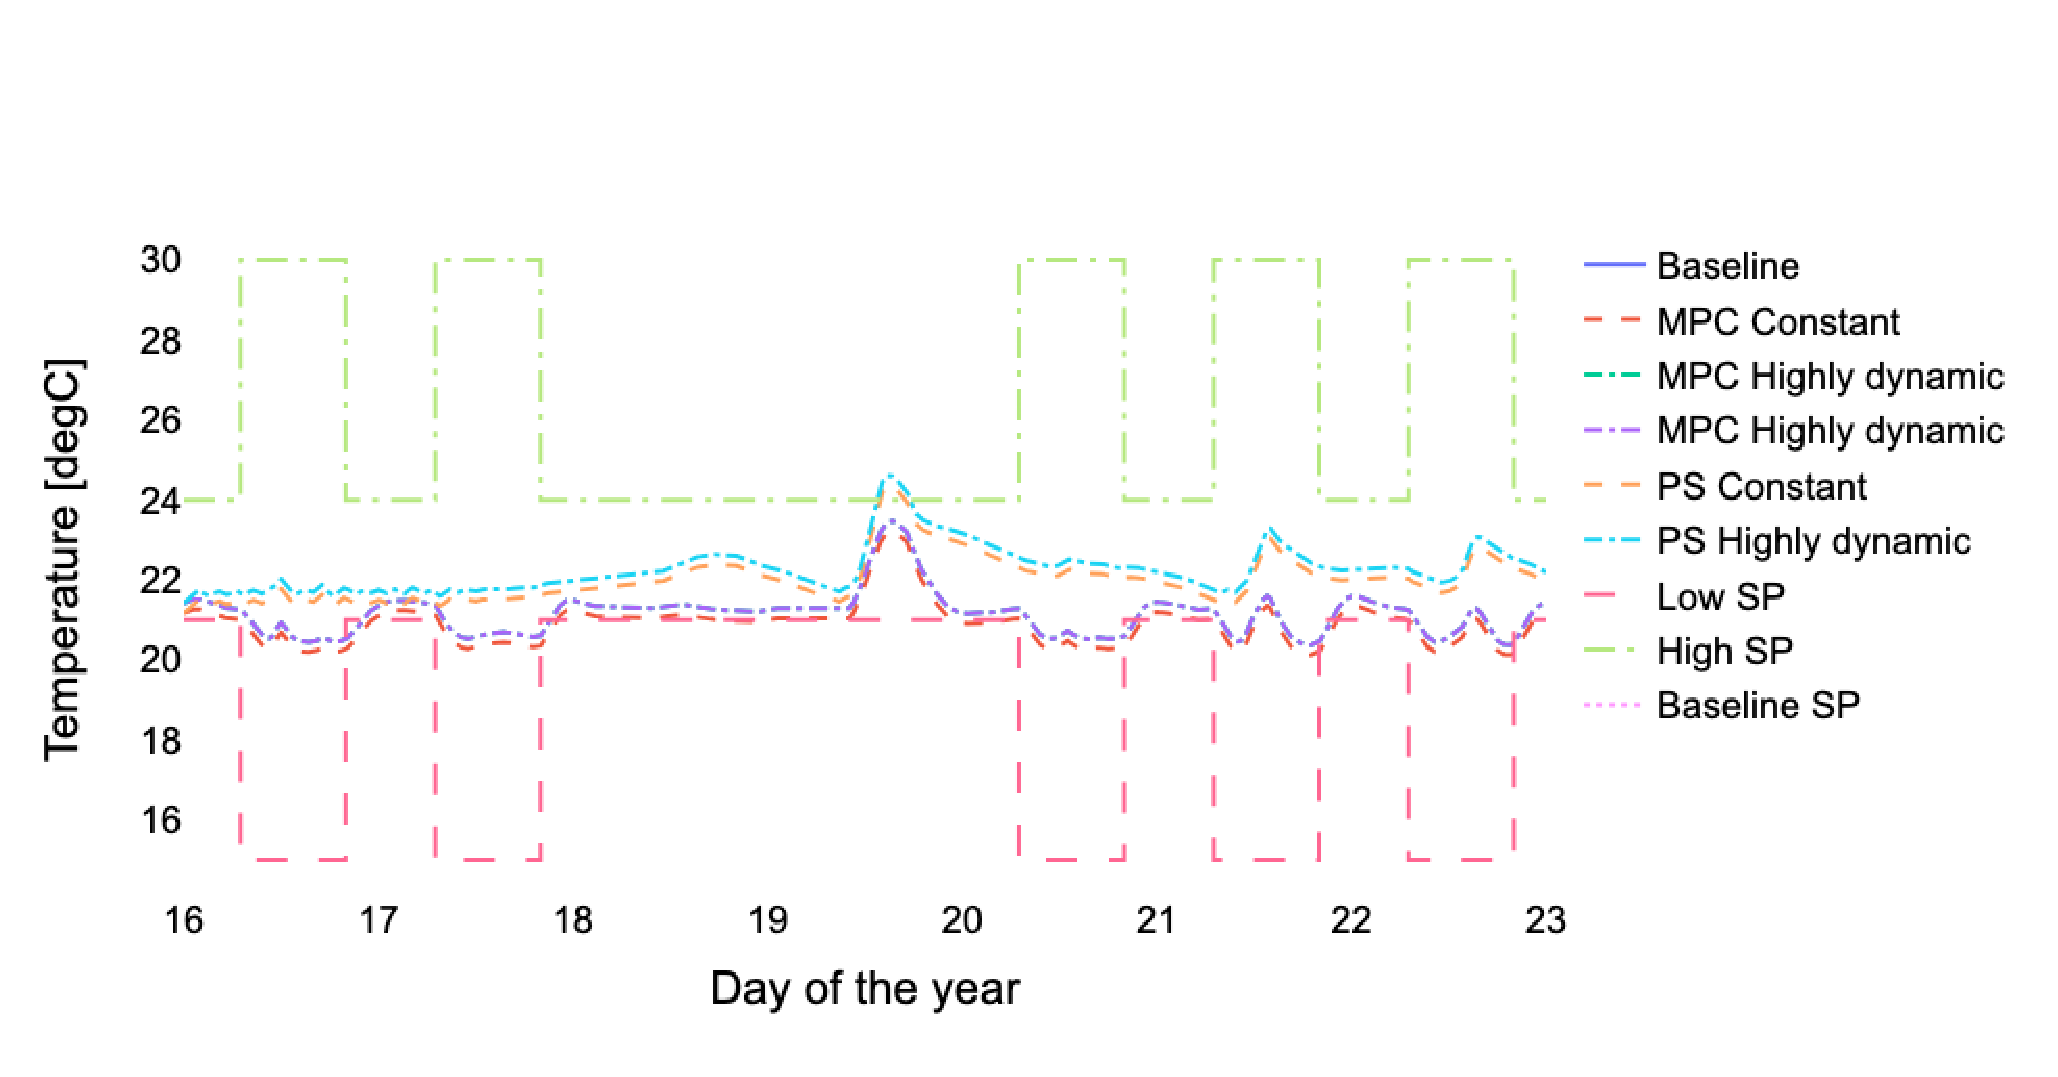
\includegraphics[scale=.4]{boptest/Fig4.eps}
% figure caption is below the figure
\caption{Timeline of indoor zone temperature for each controller}
\label{fig:4}       % Give a unique label
\end{figure}
%

The evolution of the thermal discomfort along the simulation for the baseline controller and the MPC in the three price scenarios is shown in Figure \ref{fig:5}. The evolution of the program synthesis is left out from the figure for clarity.
\begin{comment}
% For one-column wide figures use
\begin{figure}
\includegraphics[scale=.4]{boptest/Fig5.eps}
% figure caption is below the figure
\caption{Thermal discomfort for the baseline and the three MPC scenarios in the typical heat day simulation.}
\label{fig:5}       % Give a unique label
\end{figure}
%

Figure \ref{fig:6} represents the evolution of the energy cost for the same simulations.

% For one-column wide figures use
\begin{figure}
  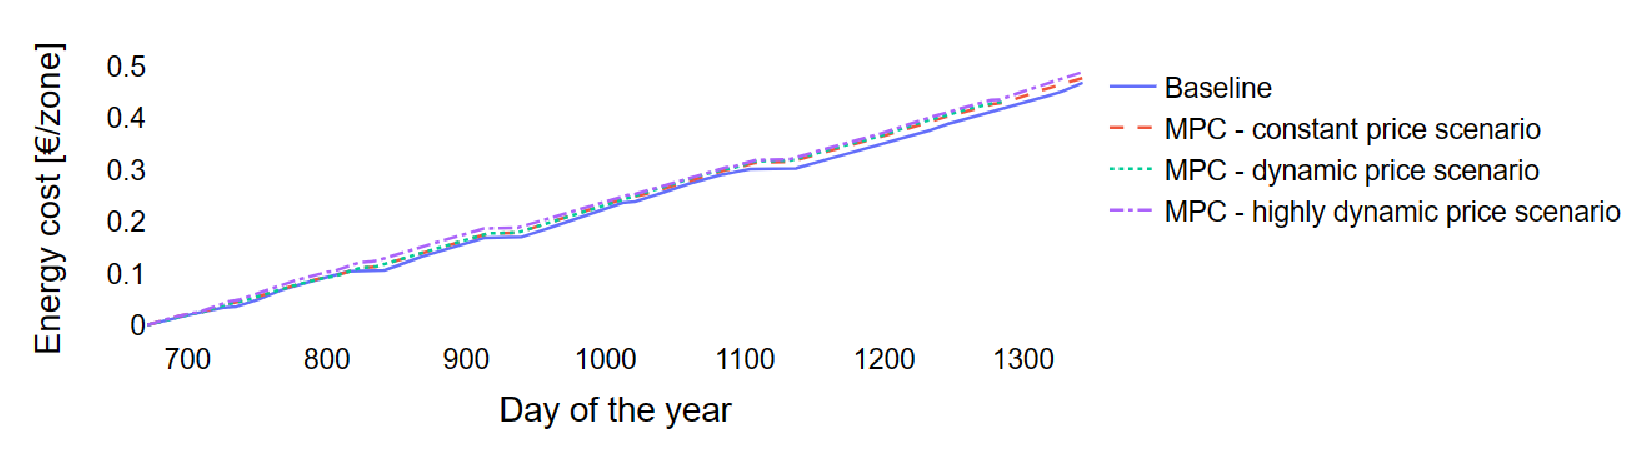
\includegraphics[scale=.4]{boptest/Fig6.eps}
% figure caption is below the figure
\caption{Evolution of the energy cost for the baseline and MPC with different electricity price schemes for a typical heat day week.}
\label{fig:6}       % Give a unique label
\end{figure}
%


\subsection{Typical heat day period simulations}
\label{'results_typical'}
The second week from the typical heat day period was simulated for the baseline, the MPC and the program synthesis. Both the MPC and program synthesis were run for the three electricity price scenarios. As the baseline controller's logic is independent from the pricing scheme, its performance is not influences by the prices, and thus just a simulation of the baseline controller is considered for each period. Table \ref{tab:3} depicts the KPI corresponding to each simulation.

\begin{table}
    \caption{Overview of KPI of each controller in the typical heat day period.}
    \label{tab:3}
    
    \centering
    \begin{tabular}{lllllll}
        \hline
        \noalign{\smallskip}
        Controller & Price Scenario & Thermal Discomfort [K·h/zone] & Energy Use [kWh/m2] & Energy Cost [€/m2] & Emissions [kgCO2eq/m2] \\
        \noalign{\smallskip}
        \hline
        \noalign{\smallskip}
        Baseline & - & 4.385 & 1.766 & 0.448 & 0.295 \\
        MPC & Constant & 0.156 & 1.232 & 0.310 & 0.205 \\
        MPC & Dynamic & 0.148 & 1.224 & 0.312 & 0.205 \\
        MPC & Highly dynamic & 0.147 & 1.232 & 0.289 & 0.206 \\
        Program synthesis & Constant & 20.450 & 1.205 & 0.305 & 0.201 \\
        Program synthesis & Highly dynamic & 20.450 & 1.205 & 0.305 & 0.201 \\
        \noalign{\smallskip}
        \hline
    \end{tabular}
\end{table}


The MPC shows an overall improvement in the thermal comfort with respect to the baseline controller in the three scenarios, as well as a reduction in energy use, energy cost and CO2 emissions. The thermal discomfort decrease compared to the baseline is of 96.44\% for the constant price scenario, 96.62\% when the price is dynamic, and 96.65\% for highly dynamic prices. The energy use savings range between 30.23\%-30.7\%, the energy cost reduction is very similar, being 30.8\%, 30.36\% and 35.5\% for constant, dynamic and highly dynamic respectively. CO2 emissions reduction are also achieved, up to 30.16\% in the most favourable scenario.

In the case of program synthesis, the thermal discomfort is 78.56\% greater than with the baseline controller. On the other hand, the energy use reduction is up to 31.77\%, the energy cost is 31.91\% lower with program synthesis and the emissions are also 31.86\% lower.

The evolution of the indoor zone temperature along the simulation for the baseline controller, the MPC and program synthesis in the three price scenarios is shown in Figure \ref{fig:4}. The baseline setpoint is depicted, which is equal to 21.2ºC during occupation hours, and it is lowered to 20.2ºC when there are no occupants. The low and high limits that are used to calculate the thermal discomfort are also depicted in Figure \ref{fig:7}.

% For one-column wide figures use
\begin{figure}
  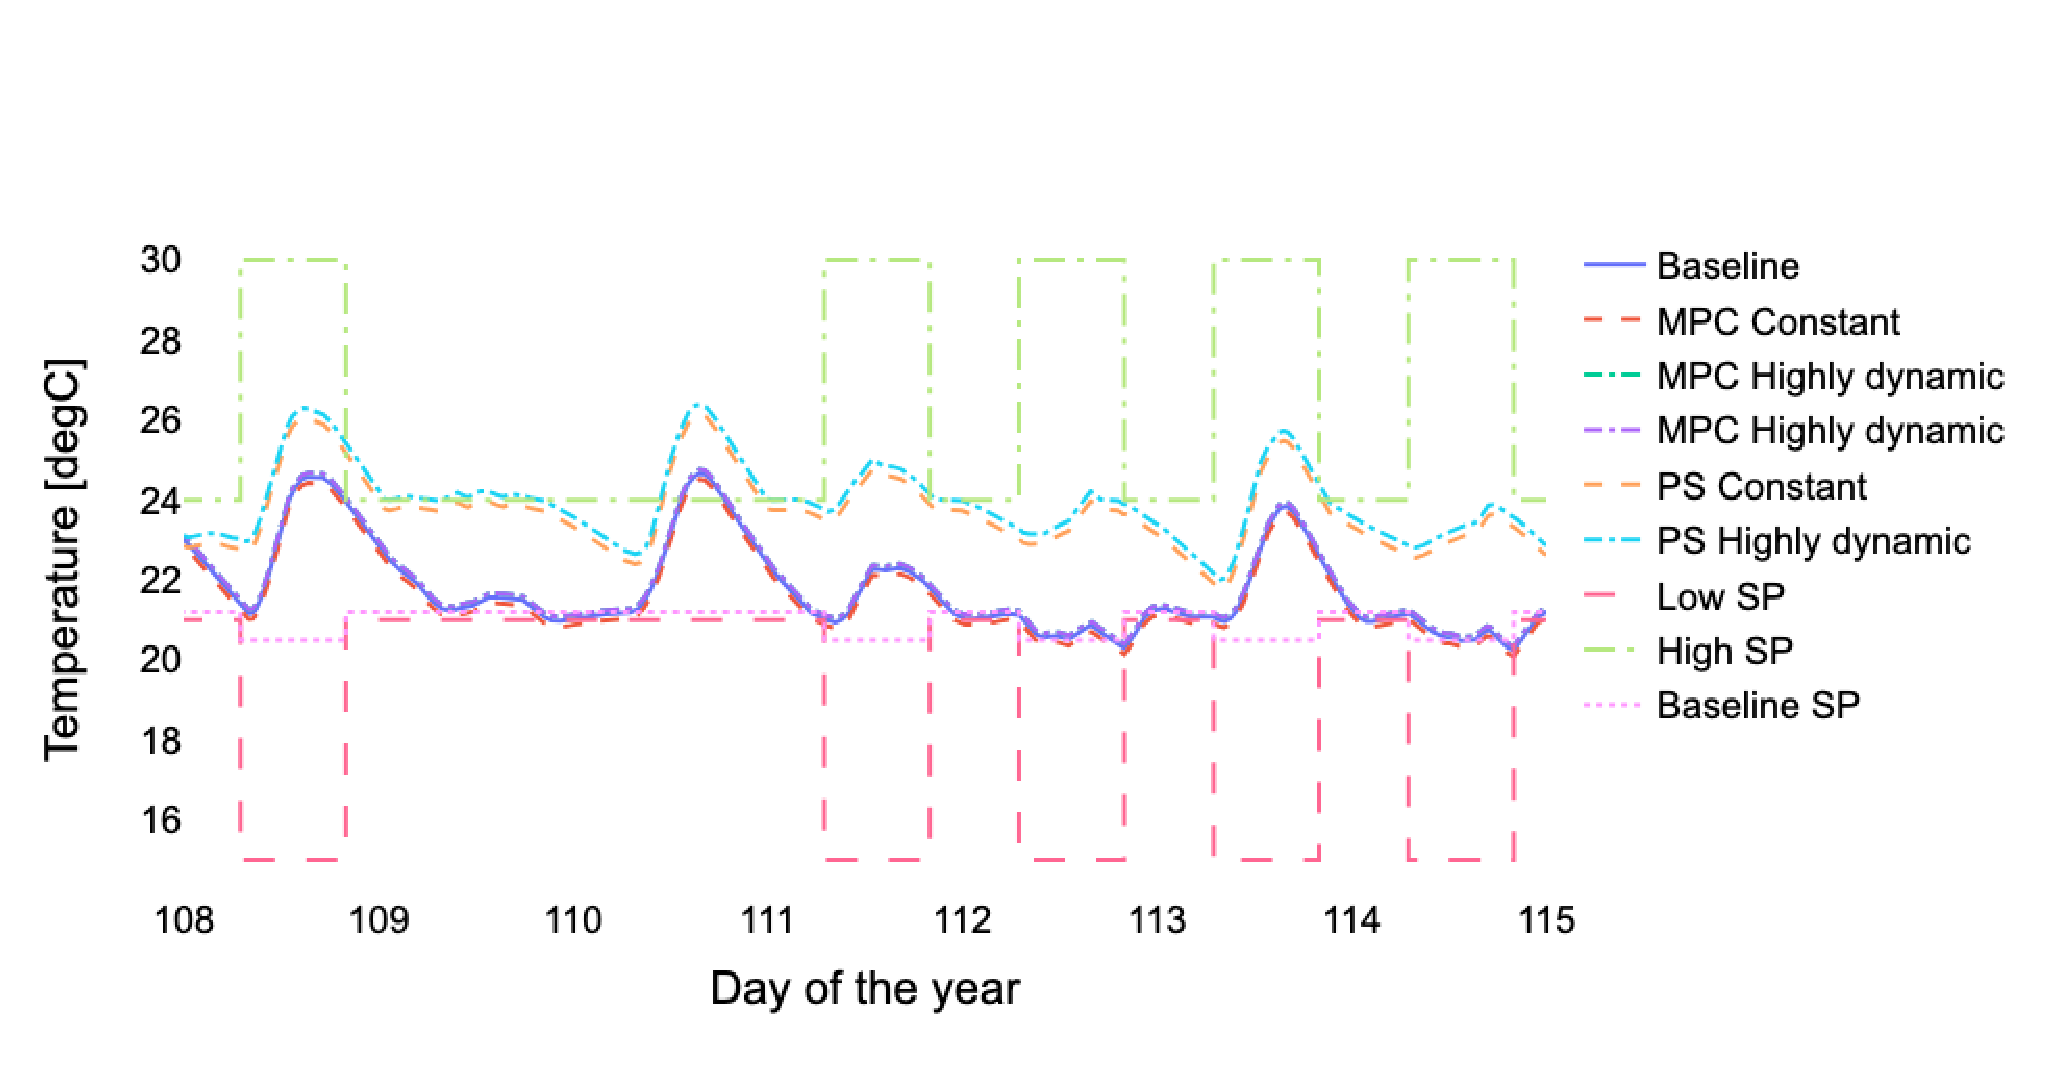
\includegraphics[scale=.4]{boptest/Fig7.eps}
% figure caption is below the figure
\caption{Indoor zone temperature through the simulation for the baseline, the MPC and program synthesis in typical heat period, together with the lower and upper comfort limits and temperature setpoint for baseline controller.}
\label{fig:7}       % Give a unique label
\end{figure}
%


The evolution in the thermal discomfort corresponds to this cumulative thermal discomfort along the simulation, depicted in Figure \ref{fig:8}.

% For one-column wide figures use
\begin{figure}
\includegraphics[scale=.4]{boptest/Fig8.eps}
% figure caption is below the figure
\caption{Thermal discomfort for the baseline and the three MPC scenarios in the typical heat day simulation.}
\label{fig:8}       % Give a unique label
\end{figure}
%

The performance of the MPC compared to the baseline for the second objective, which is the reduction is cost, is reflected in Figure \ref{fig:9} which depicts the energy cost accross the simulation.

% For one-column wide figures use
\begin{figure}
  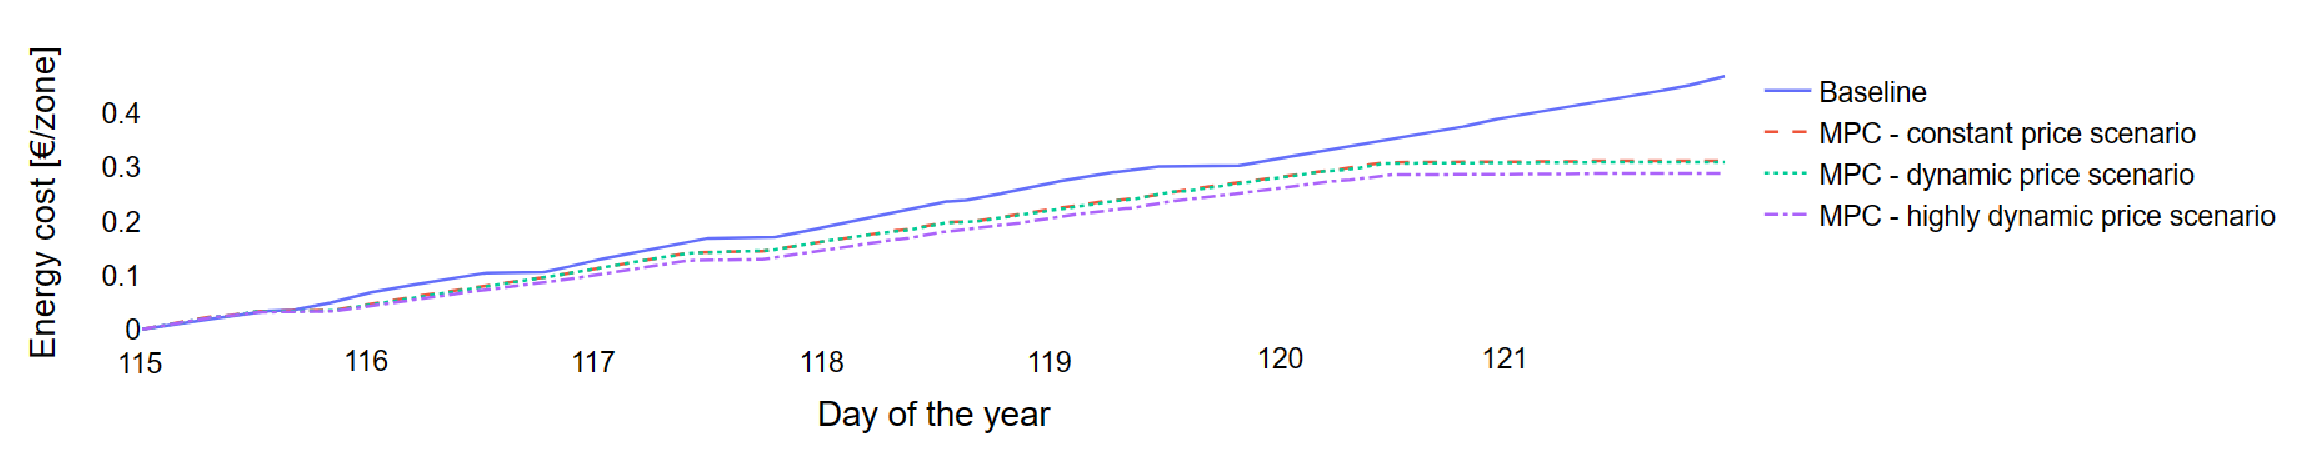
\includegraphics[scale=.4]{boptest/Fig9.eps}
% figure caption is below the figure
\caption{Evolution of the energy cost for the baseline and MPC with different electricity price schemes for a typical heat day week.}
\label{fig:9}       % Give a unique label
\end{figure}
\end{comment}

\section{Discussion}
\label{sec:discussion}
First, a discussion analysing the results described in \ref{sec:results} is included. Then, a more general discussion is included comparing both methdoologies based on this research study.

\subsection{Outcomes from the simulations with the bestest hydronic heat pump emulator}

Table \ref{tab:2} presents evidence that the MPC demonstrates efficacy in enhancing thermal comfort assurance, resulting in a reduction of overall discomfort to less than 0.5K·h/zone across three distinct electricity pricing scenarios when contrasted with the 4.385K·h/zone associated with the baseline controller. Conversely, other KPIs yield less favorable outcomes when employing the MPC in this period. It is essential to highlight that the enhancement in thermal comfort comes at the cost of increased energy consumption, consequently leading to heightened energy expenditures and emissions.

It is noteworthy that the disparities in energy-related KPIs (usage, cost, and emissions) are relatively modest. Specifically, the escalation in energy cost is a mere 3.14\%, with the cost rising by 2.23\%, and emissions increasing by 2.15\% in the constant electricity price scenario. These values exhibit remarkable similarity in the other two scenarios. Nonetheless, the MPC demonstrates a noteworthy 89\% improvement in thermal discomfort under constant pricing conditions. Consequently, the MPC succeeds in ensuring thermal comfort with comparable energy utilization.

The distinctive advantage of implementing the MPC on peak heat days lies in its capability to ensure thermal comfort with a similar energy consumption. This underscores the MPC's ability to strike a balance between enhanced comfort and energy efficiency, particularly during periods of heightened thermal demand.

In the realm of program synthesis, an observation akin to the behavior exhibited by MPC during peak heat periods emerges. Notably, both program synthesis and MPC demonstrate a congruent tendency wherein thermal comfort experiences and enhancement. However, a nuanced distinction arises in the degree of improvement, with MPC showcasing a more pronounced impact compared to program synthesis. It is noteworthy that this amelioration in thermal comfort is achieved at the expense of a marginal escalation in energy consumption, associated costs, and emissions.

When typical heat periods are analyzed, the results described in \ref{'results_typical'} show that the MPC can outperform the operation with a baseline controller for the three pricing scenarios in terms of thermal comfort, energy use, energy cost and CO2 emissions. 

First and foremost, the MPC can reduce the thermal discomfort (see \ref{fig:8}) by tracking more accurately the indoor zone temperature \ref{fig:7}. This is due to its capacity to predict the evolution of the indoor temperature based on the predicted boundary conditions and the operation possibilities. This advantage is very helpful when facing sudden changes on the temperature setpoints. Figure \ref{fig:7} shows how the indoor temperature differs more from the desired setpoint when a sudden change in the setpoint occurs with the baseline controller. In addition, the MPC, as it is implemented through a dynamic optimization that incorporates the objective of minimizing the energy cost, it is able to improve the KPI related to energy cost, emissions and energy use. The MPC focuses just on minimizing the energy cost, by adjusting the heat pump operation to the hours with the lowest price as far as the thermal comfort is not compromised. Moreover, the MPC also seeks to reduce the energy consumption as this decreases the energy cost too. In this sense, as the heat pump COP model is embedded in the MPC, it can also consider how to operate the heat pump in a more efciient way while covering the demand. This is reason why the energy use is also improved as well as the associated CO2 emissions.

Regarding the three pricing scenarios for which the MPC is simulated, the constant pricing scenario reduces the energy cost by the improvement in the performance of the heat pump and consequently the associated energy saving. In the dynamic pricing scenario, the capacity to reduce the energy cost increases as the variable prices aid to shift the consumption to the favourable hours. However, as it can be seen in \ref{fig:8}, this difference is not very notable. Nevertheless, the highly dynamic pricing schemes widens up the energy cost reduction possibilities, becoming the scenario that gets the highest energy cost reduction.

It should be noted that the baseline controller embedded in BOPTEST already presents an operation strategy with a low energy consumption, as the setpoint is set to 21.2ºC (the lowest possible setpoint to avoid thermal discomfort) and even lower when there are no occupants in the room.

In the evaluation of program synthesis in comparison to the baseline controller for typical heat days, a noteworthy revelation emerges, indicating a capacity for program synthesis to effectuate reductions in energy consumption, cost, and emissions. Intriguingly, these reductions manifest in percentages strikingly similar to those attained by the MPC counterpart. However, a pivotal distinction surfaces in the domain of thermal comfort, where program synthesis falls short. Despite its commendable achievements in energy-related metrics, the synthesis approach appears to grapple with a trade-off, compromising thermal comfort to achieve these savings. The inability to concurrently optimize both thermal comfort and energy-related objectives highlights a crucial limitation in the methodology, suggesting the need to include an additional functionality or explanation through large language models that enables an harmonious balance between the two paramount objectives.

Furthermore, the observed parallelism in the percentage reductions of energy use, cost, and emissions between program synthesis and MPC underscores the efficacy of program synthesis in mitigating environmental impact and resource consumption. Yet, the imperative to acknowledge the nuanced trade-off with thermal comfort emphasizes the necessity for further refinement and exploration of alternative strategies that may harmonize these seemingly conflicting objectives in the pursuit of more holistic and sustainable control systems.


\paragraph{Preliminary comparison of the methodologies based on the simulations.}

The efficacy of Model Predictive Control (MPC) becomes evident in its ability to consistently deliver the desired performance across varying conditions. During typical days and throughout a typical heating period, MPC excels in guaranteeing thermal comfort while concurrently reducing energy cost, subsequently leading to a reduction in overall energy use and emissions. This success underscores MPC's capability to holistically optimize the indoor environment, balancing the comfort of occupants with the imperative to minimize energy consumption and associated environmental impacts.

When faced with extreme peak conditions, MPC continues to demonstrate its prowess by ensuring thermal comfort, a feat unattainable by the baseline controller. While this achievement is coupled with a slight increase in energy use, the magnitude of this increase is negligible. This suggests that MPC is well-equipped to adapt to challenging scenarios, making it a reliable choice for maintaining indoor comfort even under the most demanding environmental conditions.

Program Synthesis emerges as an intriguing alternative to MPC, particularly evident in the highly dynamic pricing scenario during peak heat days. While it demonstrates similarities to MPC in enhancing thermal comfort, it is important to note that the results, albeit promising, fall slightly short of the performance achieved by MPC. In this particular scenario, program synthesis showcases an increase in thermal comfort at the expense of a marginally higher energy cost for peak heat period. However, program synthesis also demonstrates that is able to reduce the energy cost, as well as the use and emissions, when typical conditions are considered, but in exchange for a loss in thermal comfort. 

However, challenges persist in making program synthesis adaptable across all scenarios. As mentioned above, the simulations crashed for the dynamic pricing scenarios, which should be similar to the highly dynamic scenario. This indicate that the methodology may present some challenges when scaling to other use cases, specially when changes in the boundary conditions occur. Despite this limitation, the winning program generated for a particular case (peak heat period with highly dynamic price) showed that can work in other circumstances achieving the original targets: this winning program can also improve thermal comfort when the pricing schemes change with respect to the reference case, and can reduce energy cost, use and emissions when the conditions are typical, not so extreme. As the original weighting to balance the two objectives was done for the reference case, this may be the source of having unbalance between the two objectives in the typical heat days, reaching an unbalanced trade-off that produces significant energy savings in exchange of loss of thermal comfort.

\subsubsection{Remarks about opportunities, challenges and barriers of MPC and program synthesis based on the study}

There are some additional aspects, apart from the results obtained in the simulation, that need to be considered when comparing the two approaches.

\paragraph{Development effort}
The first aspect to be analyzed is who is required for the development of each approach. 
Developing an MPC for building applications demands a multidisciplinary skill set, particularly a profound understanding of energy systems encompassing buildings, heat/cold production units, and HVAC. The ability to intricately model these systems is paramount. Simultaneously, a grasp of building dynamics and physics is vital. Expertise in control and dynamic optimization is also essential. Despite the emergence of user-friendly tools aiding in optimization and MPC, some programming skills remain necessary. 

In contrast, program synthesis for building control leans heavily on skills related to computer science, software engineering, and formal methods. Unlike MPC, extensive knowledge of the specific building system is not mandatory. Deploying a program synthesis solution, as described in this chapter, demands a comparable amount of effort and time to MPC development due to its innovative nature.

The difference in the development effort may rely on the replication of the solution for a different building. Even if future research needs to be conducted to further investigate this point, some preliminary conclusions can be extracted from this work. Implementing MPC is time-consuming, requiring adaptation to each unique use case. Although recent efforts have focused on addressing this issue, replication and scalability remains a significant challenge in MPC for buildings. In the case of program synthesis, the way to build the program through a more comprehensive description makes it easier to be replicated for different use cases once the configuration to build the program is ready. The major change when using the methodology applied in this chapter to a different emulator is the description of the desired program.

\paragraph{Deployment requirements}
Deploying an MPC requires a considerable computational capacity, as a dynamic optimization problem is solved at each execution step, that is, usually every 15 minutes or one hour. Sufficient computational resources, including processing power and memory, are necessary to perform these calculations in real-time. This implies additional deployment cost and resources.

In the case of program synthesis, the execution performed to calculate the program giving the best solution, denoted as the winning program, also requires a high computational cost. Moreover, it still encounters the limitation on computational capacity to consider larger periods of operation data to train the models. Despite this limitation, an interesting finding of the work is that the winning program generated by program synthesis for this emulator required less computational cost than the MPC. This could open possibilities in the future to generate programs that can be deployed in the current control systems with no strict requirements of computational capacity as it is the case of the MPC.

\section{Conclusions}
\label{sec:conclusion}
This chapter presents a comparison between a widely used technique in research of buildings optimal operation, that is, MPC, and program synthesis with large language model, a promising technique which has been applied to other fields but has not been tested for buildings yet. The comparison is performed using the BOPTEST framework, which enables simulating different controllers with the same testbench and boundary conditions, obtaining KPIs that are directly comparable. As a test case, a bested hydronic heat pump for a single thermal zone dwelling is chosen, with a peak heat time period of one week and a dynamic pricing scenario. The MPC is developed using a grey-box reduced order model that is recalibrated at each step with the latest available measurements of the system using the MHE estimation technique. The cost function of the MPC tackles to reduce the energy cost as well as assuring the thermal comfort. 

The MPC exhibits a notable capacity to enhance thermal comfort within the confines of a typical heat demand week, achieving enhancements of up to 96.62\%. Additionally, MPC yields substantial reductions in energy costs, ranging between 30.8\% and 35.5\%, contingent upon the specific price scheme employed. The most significant reduction in energy costs is observed in the highly dynamic price scenario. In simulations with extreme heat conditions, MPC successfully improves thermal comfort, albeit with a marginal increase in both energy use and associated costs.

During the peak heat week, program synthesis exhibits a commendable ability to yield results comparable to those achieved by MPC. However, a discernible disparity surfaces in the extent of improvement in thermal comfort, with the MPC outperforming program synthesis in this specific context. This discrepancy suggests that while program synthesis demonstrates versatility and efficacy in various scenarios, its optimization may require a nuanced understanding of specific environmental conditions. In the evaluation of typical heat days, program synthesis once again demonstrates its prowess in significantly reducing energy costs, consumption, and emissions, mirroring the achievements of MPC. Nevertheless, a noteworthy challenge arises in the optimization of thermal comfort, wherein issues related to the weighting of objectives become apparent. The utilization of a winning program designed for a particular scenario in disparate conditions underscores the high adaptability of program synthesis but also highlights the importance of tailoring its parameters to diverse contexts. These preliminary findings unveil intriguing facets of program synthesis, emphasizing the need for nuanced parameterization and scenario-specific optimization to unlock its full potential in achieving a harmonious balance between energy efficiency and thermal comfort.

\section{Abbreviations}
\renewcommand{\labelitemi}{}
\begin{itemize}
    \item{$BOPTEST$: Building Optimization Testing Framework}
    \item{$CAPFT$: Capacity modifier function with temperature}
    \item{$CO2$: Carbon dioxide}
    \item{$EIR$: Energy input ratio}
    \item{$EIRFT$: Energy input ratio function with temperature}
    \item{$EIRFPLR$: Energy input ratio function with partial load ratio}
    \item{$GPT$: Generative Pre-trained Transformers}
    \item{$HVAC$: Heating Ventilation Air Conditioning}
    \item{$IDEAS$: Integrated District Energy Assessment Simulations}
    \item{$IPOPT$: Interior Point Optimizer}
    \item{$KPI$: Key Performance Indicator}
    \item{$MHE$: Moving Horizon Estimator}
    \item{$MPC$: Model Predictive Control}
    \item{$PI$: Proportional Integral}
    \item{$PLR$: Partial load ratio}
    \item{$PS$: Program synthesis}
    \item{$RC$: Resistance capacitance}
    \item{$RL$: Reinforcement Learning}
\end{itemize}

 

\section{Symbols}

\begin{itemize}
    \item{$C$: Thermal capacitance, kWh/(ºC)}
    \item{$\eta$: Efficiency}
    \item{$P$: Power, W}
    \item{$Q$: Heat, W}
    \item{$R$: Thermal resistance, ºC/kW}
    \item{$T$: Temperature, °C}
    \item{$u$: Actuation signal, \%}
    \item{$w$: Weighting factor, -}
    \item{$x$: State variables, -}
    \item{$y$: Output variables, -}
\end{itemize}


\section{Subscripts and superscripts}

\begin{itemize}
    \item{$av$: available}
    \item{$el$: electric}
    \item{$g$: internal gains}
    \item{$hi$: higher}
    \item{$hp$: heat pump}
    \item{$lo$: lower}
    \item{$o$: outdoor}
    \item{$u$: actuation signal}
    \item{$w$: wall}
    \item{$x$: states}
    \item{$z$: thermal zone}
\end{itemize}




% Authors must disclose all relationships or interests that 
% could have direct or potential influence or impart bias on 
% the work: 
%
\section*{Declarations}
The authors declare that they have no conflict of interest.